\documentclass{article}

\usepackage{subfig}
\usepackage{float}
\usepackage{graphicx}
\usepackage{algorithm}
\usepackage{algpseudocode}
\usepackage{changepage}
\usepackage{amsmath}
\usepackage{amsthm}
\usepackage[driver=pdftex]{geometry}

\newtheorem{theorem}{Theorem}

\DeclareMathOperator*{\argmax}{argmax}
\DeclareMathOperator*{\argmin}{argmin}




\begin{document}
\begin{titlepage}
	
	
	\begin{center}
		\vspace{2 cm}
		{\Large \textsc{Simone Quadrelli} }
	\end{center}
	
	
	\begin{figure}[H]
		\vspace{2 cm}
		\centering
		
\includegraphics[width=0.30\linewidth]{tesiSCIENZE_TECNOLOGIE.jpg}
		
	\end{figure}
	
	\begin{center}
		\vspace{2 cm}
		{\Large \textsc{Nature-inspired Monte Carlo algorithm for the travelling salesman problem} }
	\end{center}

	\par
	\vspace{3 cm}
	
	\begin{center}
		{\large Academic year 2019 - 2020}
	\end{center}
\end{titlepage}

\pagenumbering{gobble}
\newpage 
\pagenumbering{roman}
\tableofcontents
\listoffigures
\newpage

\pagenumbering{arabic}
\noindent \textbf{Abstract}. The aim of this project is to solve the travelling salesman problem (TSP) which consists in finding the shortest hamiltonian cycle (i.e. cycle that pass through each vertex of a graph just once) among all the vertices of a graph. \\
The problem is a \textit{NP-hard} problem and therefore there exist no feasible algorithm to solve it exactly for any possible input. The project explores the possibility to exploit simulated annealing and a genetic algorithm to compute with adequate approximation the shortest hamiltonian cycle.\\
The report shows the result of the simulations computed on some cities of northern Italy and compares the exact feasible solutions with the approximated ones. It also provides an analysis of the computational time needed to obtain an exact optimal solution and to obtain an approximately optimal solution.
\section{Introduction}
The travelling salesman problem (TSP) consists, as mentioned before, in finding the shortest route a travelling salesman has to take to visit all the cities only once and to return to the starting point. That route is called \textit{hamiltonian cycle} in graph theory (i.e. a cycle that pass through each vertex of a graph just once), indeed the oldest and more technical formulation of the problem was proposed by sir W. R. Hamilton. \\
An algorithm that provides a solution to the travelling salesman problem can be exploited in a wide variety of applications: for instance, it can be used in logistics to optimize the path of vehicles and consequently to reduce costs. The solutions that exploit euclidean distances can easily be applied to schedule drone shipping in cities without too high skyscrapers and buildings. \\
Formally, it is possible to model the problem using an undirected, weighted and fully connected graph\footnote{For an hamiltinian cycle to exist the graph must be at least connected} $G = (N,E)$, where $N$ is the set of the cities to visit and $E =  N \times N$ is the matrix of weights. In this particular instance of the problem, the weights correspond to the euclidean distance between each couple of cities.\\
Therefore, the route of the travelling salesman is an hamiltonian cycle defined as a sequence of nodes $(n_0, .., n_{k-1})$ of length k such that $n_i \neq n_j \; \forall i,j \in \{1,..., |N|+1\}$ and $n_0 = n_{|N|+1}$. \\
\subsection{Complexity of the travelling salesman problem}
Solving the travelling salesman problem pose very tricky computational problems. Indeed, the most intuitive solution to the problem consists in computing all the possible paths and then evaluate all their lengths to find the shortest one. However, the number of possible cycles is $\frac{(n-1)!}{2}$ and grows faster than $2^n$ (i.e. $2^n = o(n!)$) and thus making it unsolvable in finite time for large $n$. Moreover, even if it was possible to generate each hamiltonian cycle in constant time, independently from their length, the algorithm will still have an exponential time complexity to find the best result.  \\
More techically, TSP is an \textit{NP-hard} problem, meaning that it is at least as hard as the hardest NP-complete problem. \textit{NP-complete} problems are problems that can be solved in polynomial time by a non-deterministic algorithm. For such a class of problem do not exist any known polynomial algorithm to solve them and may not exist. However, noone was able to prove that deterministic polynomial algorithms cannot be found.
\begin{figure}[H]
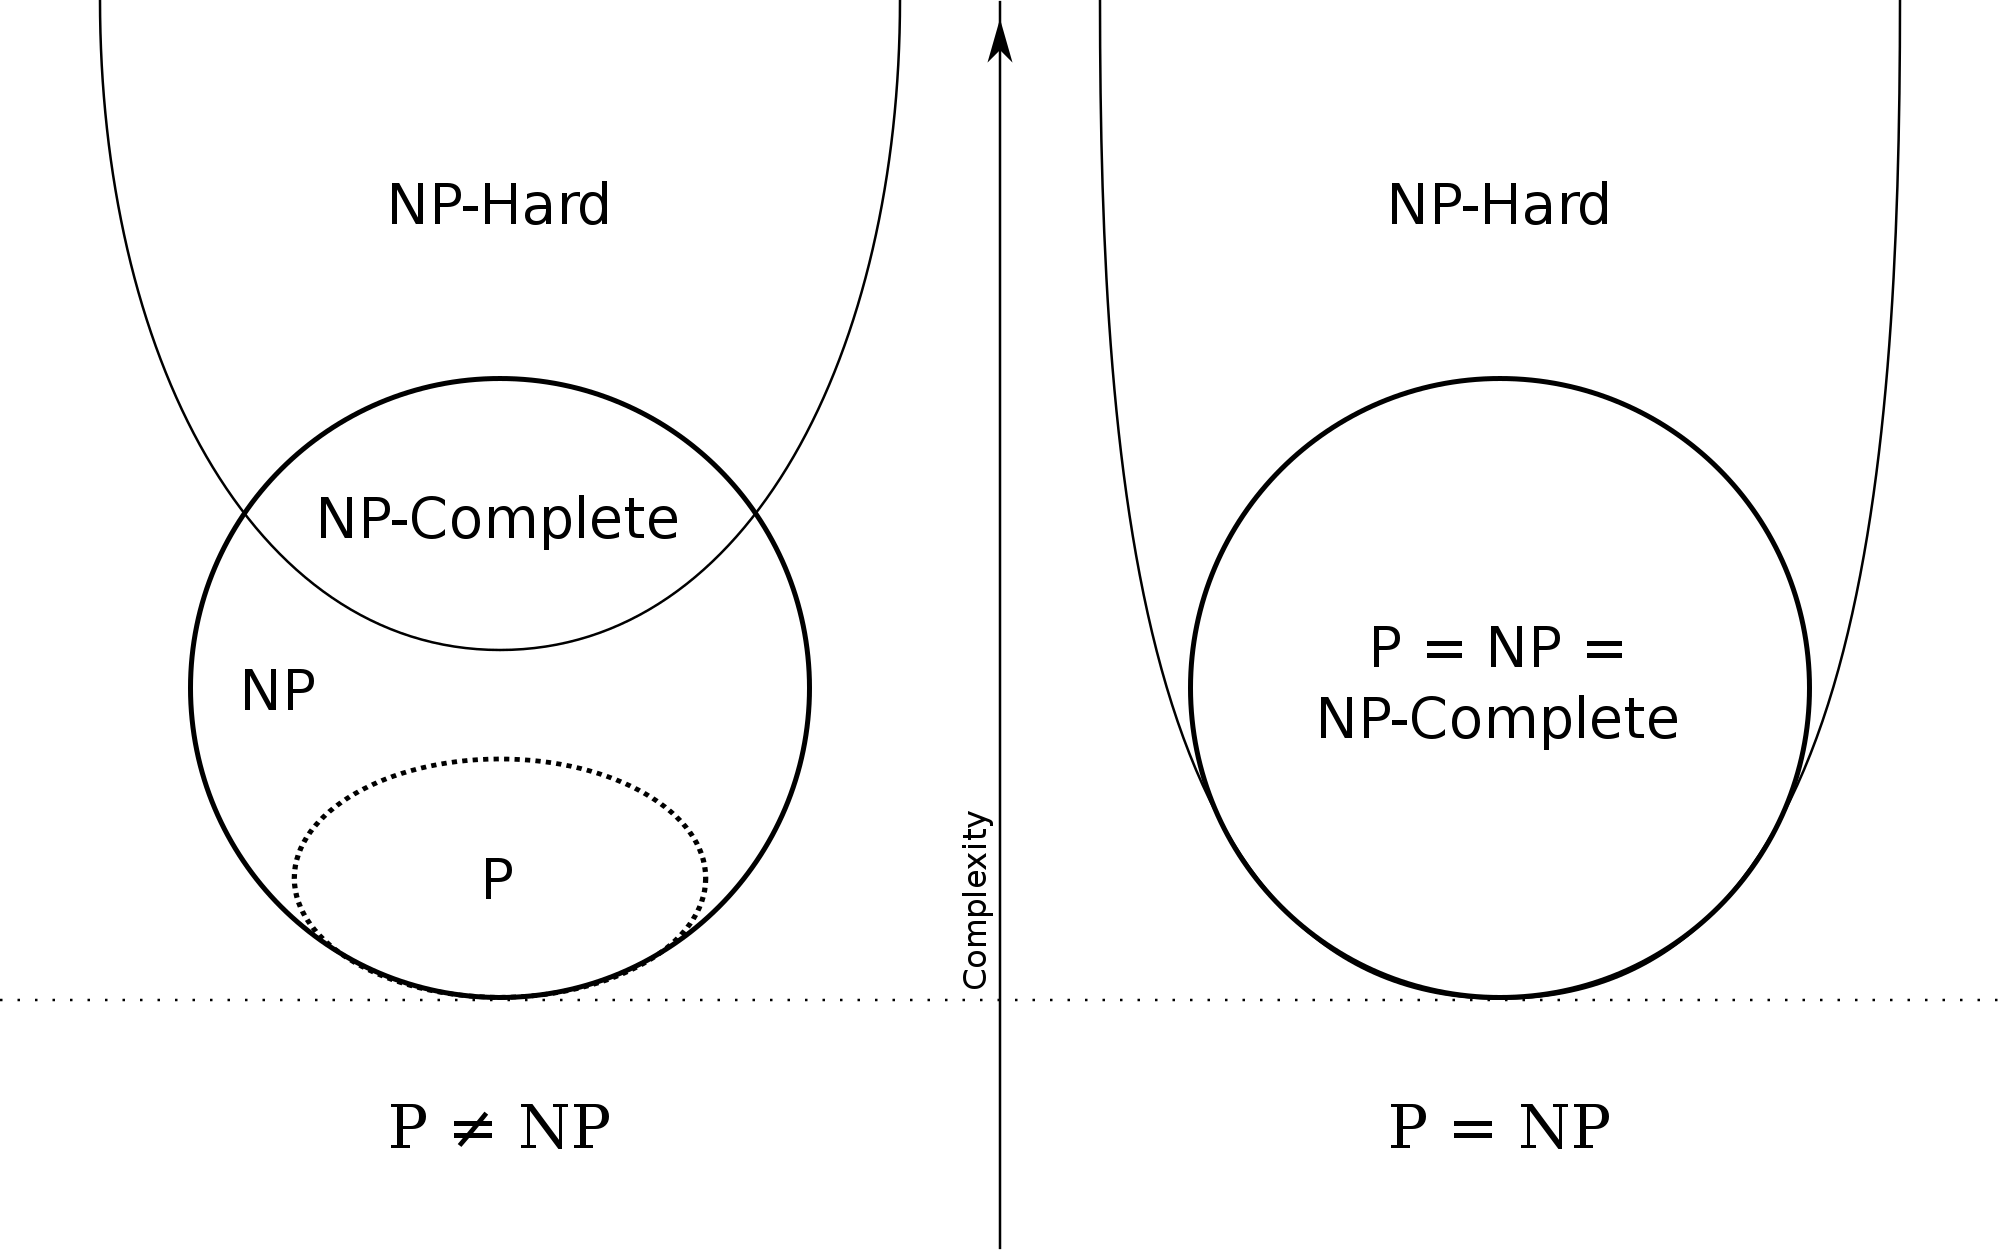
\includegraphics[scale=0.25]{complexity_classes.png} 
\centering
\caption{Computatinal complexity schema}
\end{figure}
\noindent Bearing in mind the complexity of the problem to face, the most reasonable approach relies on approximation. The technique I used to generate the possible hamiltonian cycles is a genetic algorithm, while the choice of the shortest hamiltonian cycle is done by the \textit{simulated annealing}.

\section{Literature review}
Many efforts were done to find out global optimization techniques that simulate optimization in nature. There can be depicted three main classes of algorithms:
\begin{enumerate}
\item Simulated Annealing
\item Artificial Neural Networks
\item Evolutionary Algorithms
\end{enumerate}
Among the evelutionary algorithms, there can be found different subsclasses: evolutionary programming (1962), evolution strategies (1965) and genetic algorithms (1975) that mimic in different ways Darwin's theory.  Overall, evolutionary algorithms are stochastic search algorithms simulating the natural evolution processes. \cite{gareview}\\
It was discovered that such algorithms are suitable optimization techniques for NP-hard problems and, not surprisingly, they are very fit for biological, pharmaceutical and chemical applications. \\
On the other hand, Artificial Neural Networks were exploited only recently since they require an enormous amount of data and a huge computational power. \cite{annreview} \\
Moreover, those algorithms do not provide a strightforward interpretation of their parameters and therefore may not be suitable in logistic applications.

\section{Algorithms and techniques} \label{algorithms}
This section provides a top-down overview of all the techniques and algorithms exploited. They are: Simualted Annealing, Metropolis algorithm and a genetic algorithm.

\subsection{Simulated annealing}
Simulated annealing (SA) is a technique that mimics the behaviour of heated materials slowly cooled down in metallurgy, this process decreases the impurity and increases the size of the crystals meaning that allows the materials to reach the minimum energy state. \\
It is a technique to approximate the global optimal solution when it is to be searched in an enormous space. Indeed, SA is a metaheuristic that is a general-purpose stochastic heuristic. As every metaheuristic algorithm, it relies on two principles \textit{intensitification} and \textit{diversification}. Indeed, the algorithm intensifies the search near different possible optimal solutions.\\
SA is very versatile since it does not require any prior information other than a cost function to be minimized, indeed it just supposes that states (hamiltonian cycles in this work) are distributed accordingly to the Bolzmann distribution:
\begin{equation}
e^{- \beta (cost(state))}
\end{equation}
The Boltzmann distribution is suitable to model the TSP problem since it models the distribution of states with the smallest possible bias. Indeed, its unbiasedness derives from the maximization of the Shannon's entropy, given the cost.\\
The underlying assumption of simulated annealing is that the optimal states are the states with the lowest cost, and they are reached as the temperature decreases.\\
Temperature $T$ is the inverse of $\beta$ ($T = \frac{1}{\beta}$), therefore the SA starts with low values of $\beta$ (high temperature) and, as the simulation proceeds, the values of $\beta$  increase, thus mimicking the decrease in temperature. \\
As mentioned before, the only other information needed is the cost function, that, for this specific application, is the sum of euclidean distances between the cities in the cycle, whose coordinates are expressed in longitude and latitude.\\
In the following algorithm provides a schematic overview of the simulated annealing implemented.

\begin{algorithm}[H]
    \begin{algorithmic}[1]
      \Function{simulated annealing}{\textbf{betas},number of simulations}
        \State s $\leftarrow$ generate starting state with the genetic algorithm
         \For {b in \textbf{betas}}
         	\For{n in 1,.., number of simulations}
         	 \State ns $\leftarrow$ generate a new state with the genetic algorithm starting from s
         	\State ns $\leftarrow$ METROPOLIS(s,ns,$\beta$)
         	\EndFor
        \EndFor
        \State return ns
       \EndFunction
\end{algorithmic}
\end{algorithm}

\noindent where \textbf{betas} is a set of the values of $\beta$. \\ 
The code executes all the procedures using a vectorial implementation to speed up the computation.

\subsection{Metropolis algorithm}
As SIMULATED ANNEALING algorithm above shows, Metropolis  algorithm is exploited to sample states from the Boltzmann distribution. Therefore, this section describes the algorithm and analyzes in details its properties.\\
Metropolis algorithm is a Markov Chain Monte Carlo (MCMC) algorithm used to generate values $X_n$ from a finite set of values $S$ accordingly to a target probability distribution $\pi$.  \\
The sequence of  $X_n$ can be modelled by Markov chains. Indeed, an homogeneous and finite Markov chain with state space $S$, transition matrix $P$ and initial distribution $\mu$ is a sequence of random variables $\{ X_n \}_{n \in N}$ such that
\begin{enumerate}
\item $\forall i \in S \, Pr(X_0=i)= \mu(i)$ 
\item $\forall n > 0 \; \forall i_n,...,i_0 \,  Pr(X_{n+1} = j | X_n = i_n,..., X_0=i_0) = Pr(X_{n+1} = j | X_n = i_n)$
\item $\forall n > 0 \, Pr(X_{n+1} = j | X_n = i) = p(i,j) $
\end{enumerate}
Metropolis algorithm is designed in such a way that it is very likely to move from a state with lower probability from a state with higher probability. \\
The following algorithm describes the metropolis algorithm when the target distribution $\pi$ is the Boltzmann distribution:
\begin{equation*}
\pi(\text{state}) = e^{- \beta \, \text{cost(state)}}
\end{equation*}
and $S$ is the set of all possible hamiltonian cycles with fixed length.\\
The following disseratation assumes to have generated two hamiltonian cycles (i.e states) old\_state, new\_state, whose generation is described in  section 3.3. Metropolis algorithms works as follows: if new\_state is likely to be a sample of $\pi$ it is used as new state otherwise, with a certain probability, old\_state is the current state.

\begin{algorithm}[H]
    \begin{algorithmic}[1]
      \Function{metropolis}{old\_state, new\_state, $\beta$}
      	\If {cost(new\_state) $<$ cost(new\_state)}
      	\State return new\_state
      	\EndIf
        \State threshold $\leftarrow$ unif[0,1]
        \State p  $\leftarrow min\{1,e^{- \beta (\text{cost(new\_state}) - \text{cost(old\_state}))} \}$ 
        \If {p $>$ threshold}
        	\State return new\_state
        \Else
        	\State return old\_state
        \EndIf
       \EndFunction
\end{algorithmic}
\end{algorithm}
\noindent
\subsubsection{Properties of Metropolis algorithm}
The sampling of new hamiltonian cycles is modelled by an undirected and connected graph $G = (S,E)$ whose set of states $S$ contains all the possible hamiltonian cycles and $E$ contains the transition probabilities from an hamiltonian cycle to another one. Given the graph $G$, the transition matrix $P=p(i,j)]_{i,j\in S}$ is defined as
\begin{equation}
p(i,j) =  \begin{cases} 
	0\, & \mbox{if } \{i,j\} \notin E  \\ 
	\frac{1}{d_i} \min\{1,\frac{\pi(j)}{\pi(i)}\} & \mbox{if }  \{i,j\} \in E \;,\, i \neq j\\
	1-\frac{1}{d_i} \sum_{l \in adj(i)} \min\{1,\frac{\pi(l)}{\pi(i)}\}  & \mbox{if }  i = j 
\end{cases}
\end{equation}
Since G is a connected graph, $P$ is irriducible meaning that $\forall i,j \in S \, p^n(i,j) > 0$, where $p^n(i,j) > 0$ means that exist a path of length $n$ from $i$ to $j$.\\
It can also be proved that $P$ is aperiodic \cite{metropolis}, that is: each node of the graph has a loop. More formally, the graph $G$ is aperiodic if $\forall i \in S, \,d(i)  = 1$ where
\begin{equation}
d(i) = mcd \{n \in N | \, \text{ cycle from i to i of length} \, n\}
\end{equation}
Metropolis algorithm defines a probability distribution $\pi$ that is \textit{reversible}:
\begin{equation}
	\pi(i)p(i,j) = \pi(j)p(j,i) \;\; \forall i,j \in S
\end{equation}
This is a key feature of the algorithm since a reversible distribution $\pi$ is also a stationary distribution, i.e. $\pi'P=\pi'$. This condition holds due the following theorem: 
\begin{theorem}
If a probability distribution $\pi$ is a reversible distribution for a markov chain $ \{X_n\} $, then it is also a stationary distribution.
\end{theorem}

\begin{proof}
$ (\pi'P)_j = \sum_{i \in S} \pi(i)p(i,j) = \sum_{i \in S} \pi(j)p(j,i) = \pi(j) $ 
\end{proof}
\noindent The last condition needed to assure to correctly generate the data accordingly to the target distribution $\pi$ is the uniqueness of the distribution. However, stationary distibution is unique if the transition matrix of the markov chain is primitive as stated by the follwing theorem:
\begin{theorem}
Let $\{X_n\}$ be a markov chain with a primitive (i.e. irreducible and aperiodic) transition matrix on a finite set, then  there exist only one stationary distribution and it as also the limit distribution $\lim_{n \to \infty} p^n(i,j) = \pi(j)\,  \forall i \in S$
\end{theorem}
\noindent Since $P$ is primitive, it is enough to compute the limit distribution to find the unique stationary distribution. \\
By the convergence theorem, stationary distributions can be approximated in a logarithmic number of iterations starting from any distribution. Therefore, to sample hamiltonian cycle from the stationary distribution is enough to let the simulation go on for a suitable number of iterations \cite{mctheory}, \cite{mcalgorithm}. \\

\subsection{Genetic algorithm}
To explain the functioning of the metropolis algorithm, it was assumed to have two states: new\_state and old\_state. In the following is explained how to obtain those states by the means of a genetic algorithm.\\
Genetic algorithms are a widespread class of algorithms that mimic nature. Indeed there are three fundamental operations  inspired by the theory of evolution by C. Darwin that they perform to generate new states (hamiltonian cycles). \\
Among a specie, evolution selects the fittest individuals and therefore the algorithm will chose the fittest (i.e shortest) hamiltonian cycles. \\
\begin{algorithm}[H]
    \begin{algorithmic}[1]
      \Function{selection}{\textbf{population},n\_paths}
        \State n\_parents $\leftarrow$ unif[2,n\_paths/2]
        \State order the population by fitness
        \State \textbf{fittest\_subpopulation} $\leftarrow$ extract n\_parents in order from the sorted population
        \State return \textbf{fittest\_subpopulation}
       \EndFunction
\end{algorithmic}
\end{algorithm}
\noindent The breeding of the fittest individuals produces new individuals that inherits traits from the parents, therefore the crossbreeding operation mixes some subsection of the fittest hamiltonian cycles. \\
\begin{figure}[H]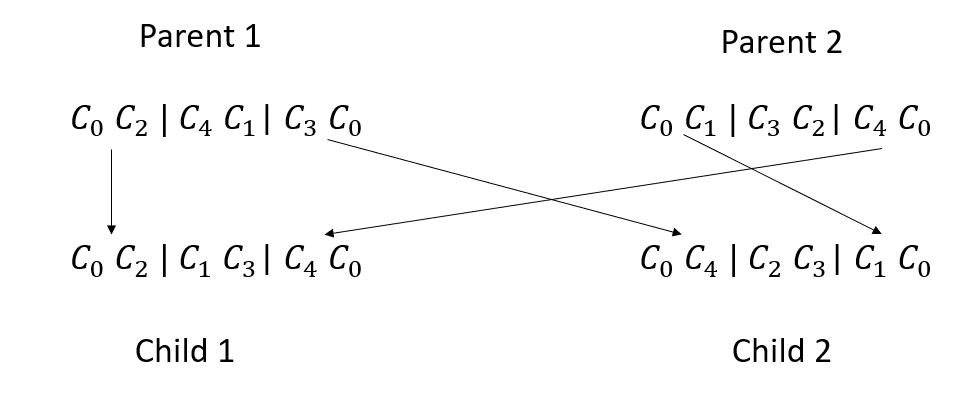
\includegraphics[scale=0.5]{crossbreeding.png} 
\centering
\caption{Crossbreeding schema}
\end{figure}

\noindent As random mutations can occur in nature but they are unlikely to, the algorithm swaps two cities with a fixed and low probability. Otherwise mutations will disrupt the optimal inherited subsequences. \\


\begin{algorithm}[H]
    \begin{algorithmic}[1]
      \Function{mutate}{\textbf{new\_population}, p}
      \For {path in \textbf{new\_population}}
        \State test $\leftarrow$ unif[0,1]
        \If {test $<$ p}
        	\State choose position1 randomly among unif[0,length of cycles-1)
  			\State choose position2 randomly among unif[0,length of cycles-1)
  			\State swap the cities in position1 and position2
        \EndIf
       \EndFor
        \State return \textbf{new\_population}
       \EndFunction
\end{algorithmic}
\end{algorithm}
\noindent To easily apply all the operations, an EVOLVE function was created.

\begin{algorithm}[H]
    \begin{algorithmic}[1]
      \Function{evolve}{\textbf{population}}
        \State \textbf{fittest\_population} $\leftarrow$ SELECT(\textbf{population})
        \State \textbf{new\_population} $\leftarrow$ CROSSBREED(\textbf{fittest\_population})
       \State \textbf{population} $\leftarrow$ MUTATE(\textbf{new\_population})
       \EndFunction
\end{algorithmic}
\end{algorithm}

\noindent There are many possible implementations of the basic operations performed by a genetic algorithm. Therefore I decided to implement them from scratch. However, the implementation of those functions is not very interesting and requires many implementative details, therefore it is omitted in the present work.

\section{Application} 
This section provides the reader with the necessary information about the choice of the distance function, the dataset and the precise algorithmical and python implementation of key functions.

\subsection{Distance}
The first problem to overcome is to choose an appropriate notion of distance. When the construction of routes faces few natural constraints, such as in the Po valley, streets are built to minimize the distance between the cities they connect. The easiest way to minimize the distance is to use the euclidean distance since small portions of earth can be considered as a plain. Therefore to realistically model the routes of the highways that connect important cities in northern Italy euclidean distance seems to be a suitable measure, as can be seen from Figure \ref{autostrade}.
\begin{figure}[H] 
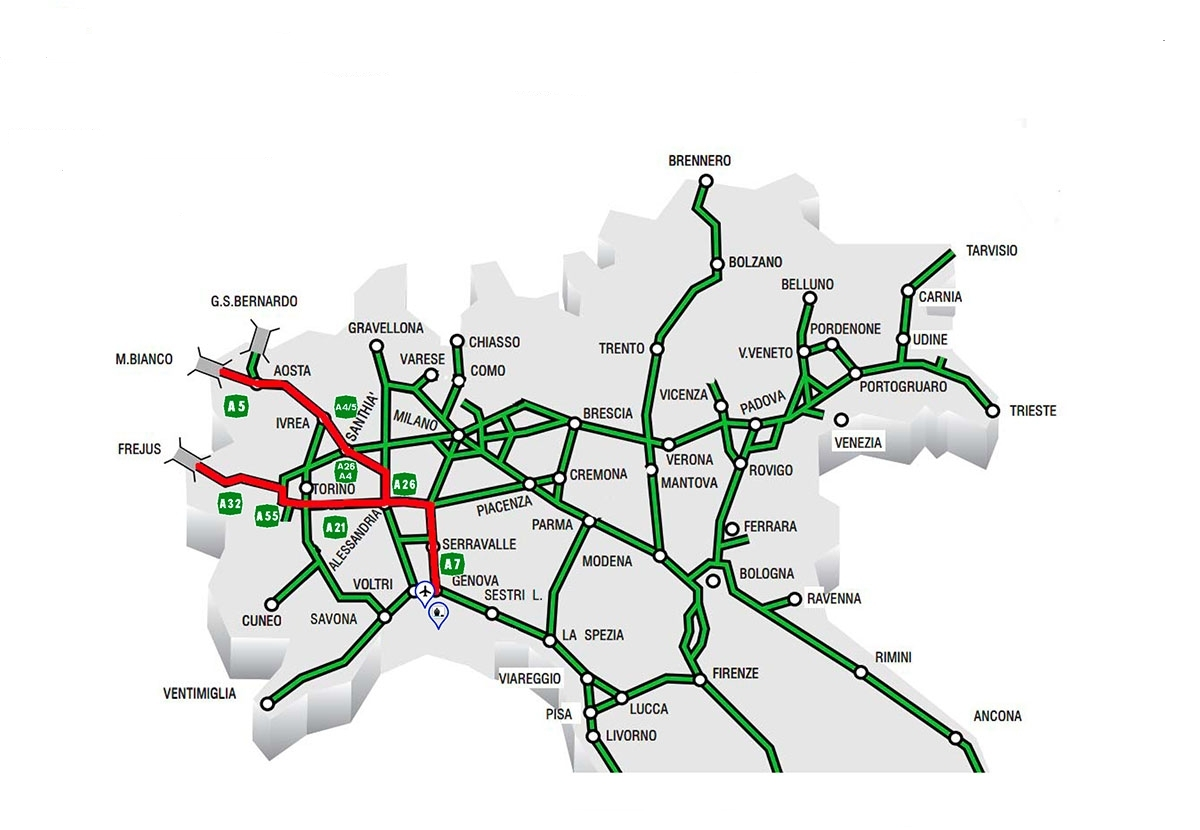
\includegraphics[scale=0.4]{autostrade.jpg} 
\centering
\caption{Scheme of the highways by \textit{Autostrade per l'Italia}\cite{autostrade}} \label{autostrade}
\end{figure}
\noindent On the other hand, euclidean distance seems not to connect too well cities in the other italian regions like Tuscany and Emilia-Romagna since the Apennine Mountains prevent to easily connect the city on the west coast of central italy to cities on the east cost.


\subsection{Dataset}
Taking into account the constraint fixed by the choice of the distance, the dataset used refers to cities in northern Italy: \textit{Varese, Novara, Torino, Milano, Como, Bergamo, Brescia, Cremona, Lecco, Lodi, Mantova, Monza, Pavia, Sondrio, Verona, Vicenza, Padova, Venezia}. \\
The dataset consists in the coordinates of the cities above in terms of latitude and longitude. Since latitude and longitude is a global scale the cities are very close one another and therefore the cost of the hamiltonian cycles is very low.\\
The information were downloaded using the python library \textit{geopy} as follows:

\begin{figure}[H]
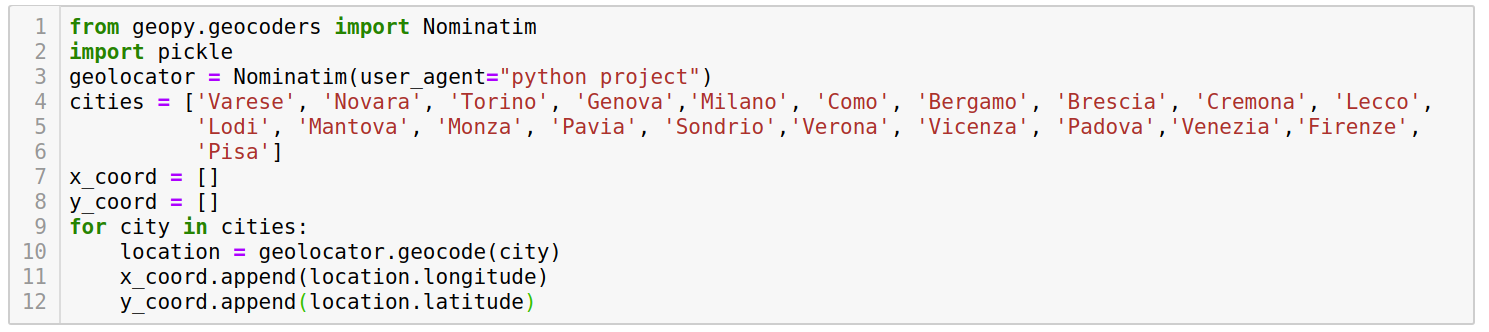
\includegraphics[scale=0.42]{download_dataset.png} 
\centering
\caption{Python code to download the coordinates of the cities}
\end{figure}

\subsection{Software used}
The objective of this simulation is to compare the optimal solutions of the TSP computed by the appromated algorithm and the exact solutions.
However, as explained before, the exact solution of the TSP is not feasible when the number of cities grows too much, therefore they are computed just as long as it is computationally feasible. \\
The algorithm select a growing set of cities each iteration, executes in parallel some predefined number of simulated annealing and select the best solution among the results of the simulated annealings. Then it computes, if feasible, the exact solution. The values are saved at each iteration and then are plotted to easily show the results.\\
The code was also instrumented to keep track of the execution time of both algorithms.
The algorithm  below provides a schematic description of the experiement run. 
\begin{algorithm}[H]
    \begin{algorithmic}[1]
      \Function{Experiment}{all\_cities}
       \For {i in 1,..., n\_cities}
       	\State  cities $\leftarrow$ all\_cities[0:i]
       	\For {for all threads}
       		\State run simluted annealing in parallel
       	\EndFor 
       	\State extract the best solution among the solutions computed by the threads
       	\If{i $<$ feasibility\_threshold}
       		\State compute the exact solution
       	\EndIf
       	\State compare the results by plotting them
       \EndFor
       \EndFunction
\end{algorithmic}
\end{algorithm}

\noindent The following python codes is the implementation of the algorithm described above. In the simulation run the starting and ending city is \textit{Varese}. \\
\begin{figure}[H]
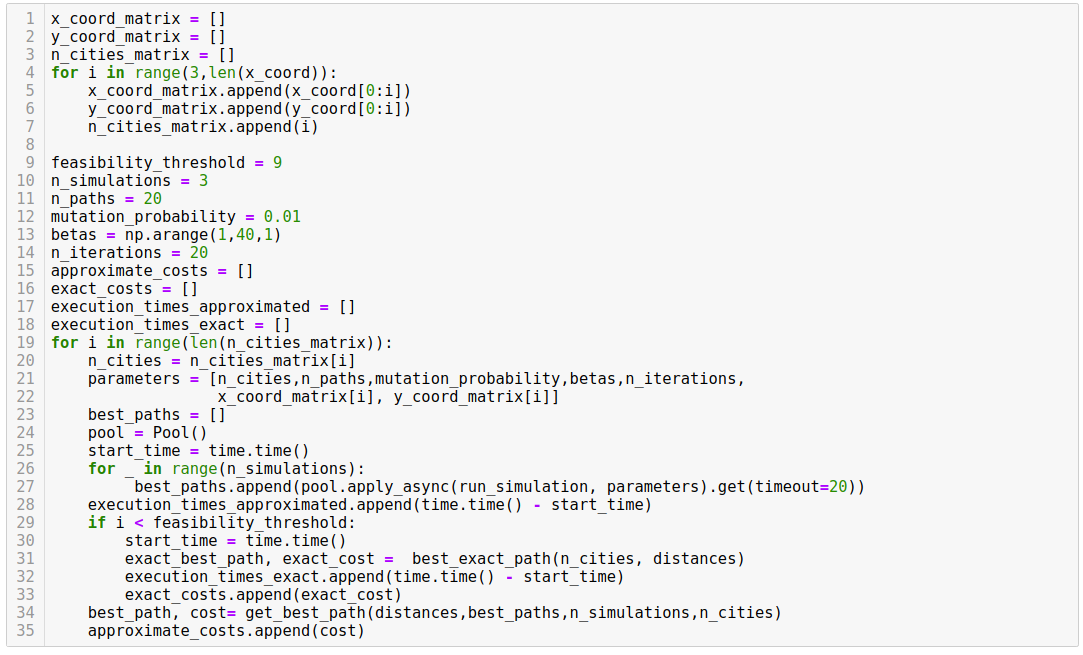
\includegraphics[scale=0.5]{simulation.png} 
\centering
\caption{Python code of the experiment}
\end{figure}

\noindent The most importan function used in the code of the experiment is RUN\_SIMULATION that executes an instance of simulated annealing. \\
The genetic algorithm generates a starting population which is a matrix then it evolves the whole population. In the end, if a cycle state is likely to come from the target distribution is accepted otherwise the evolution is rejected by Metropolis algorithm.

\begin{algorithm}[H]
    \begin{algorithmic}[1]
      \Function{run\_simulation}{\textbf{betas}, n\_iterations}
      \State generate a starting population
       \For {beta in betas}
       		\For {i in 1,...,n\_iterations}
       		\State EVOLVE the population
       		\State obtain the new state by metropolis algorithm
       	\EndFor 
       \EndFor
       \State return the shortest cycle
       \EndFunction
\end{algorithmic}
\end{algorithm}

\noindent The follwing code shows the python implementation of the algorithm explained above.
\begin{figure}[H]
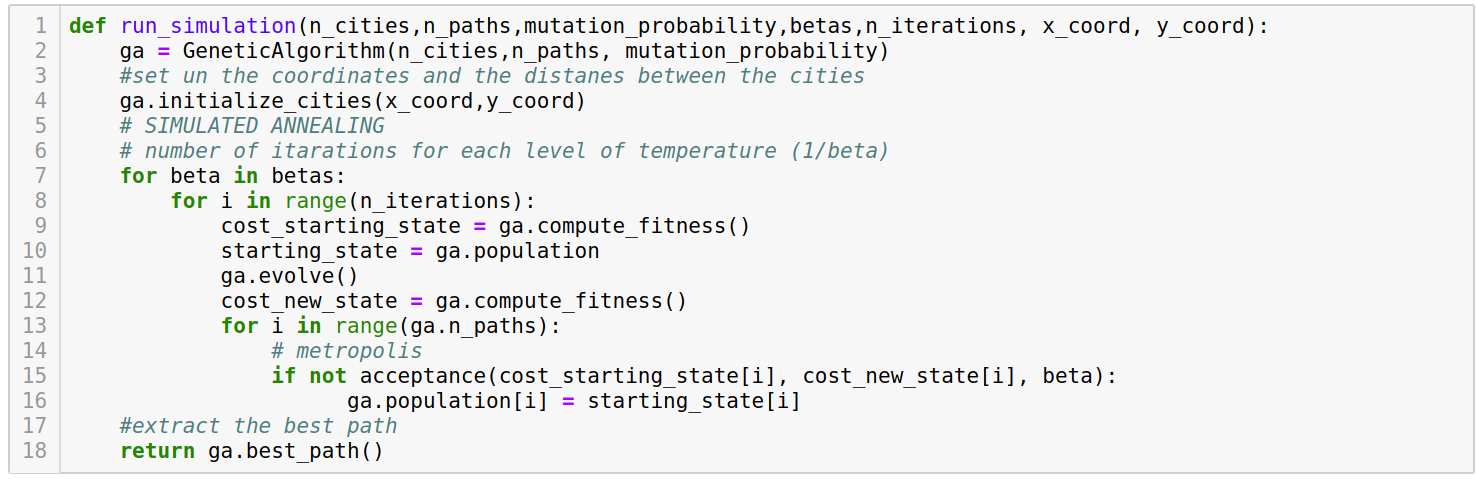
\includegraphics[scale=0.38]{run_simulation.png} 
\centering
\caption{Python code of a simulation}
\end{figure}
\noindent

\noindent A last remark, to be able to control and modify the code as wished, all the algorithms described were implemented from scratch exploiting just some support libraries such as \textit{numpy}.

\section{Results}
This section compares the simulated annealing with the exact algorithm to solve the TSP problem. \\
As expected the computational time required to compute an exact solution becomes exponentially high as the length of the cycles increases. However, for small instances of the problem, it is more efficient than the simulated annealing since it perform faster and fewer operations. On the contrary, the execution time\footnote{All time measurement rely on a Intel Core i5-7200U dual core processor and 8 GB DDR4 RAM} of the simulated annealing is almost independent from the length of the cycles and remains very low. It is worth noting that the slight variations and the peaks in the execution time plot may be caused by the scheduling of the operating system and the multithreading.
\begin{figure}[H]
\begin{adjustwidth}{-4em}{-4em}

     \subfloat{%
       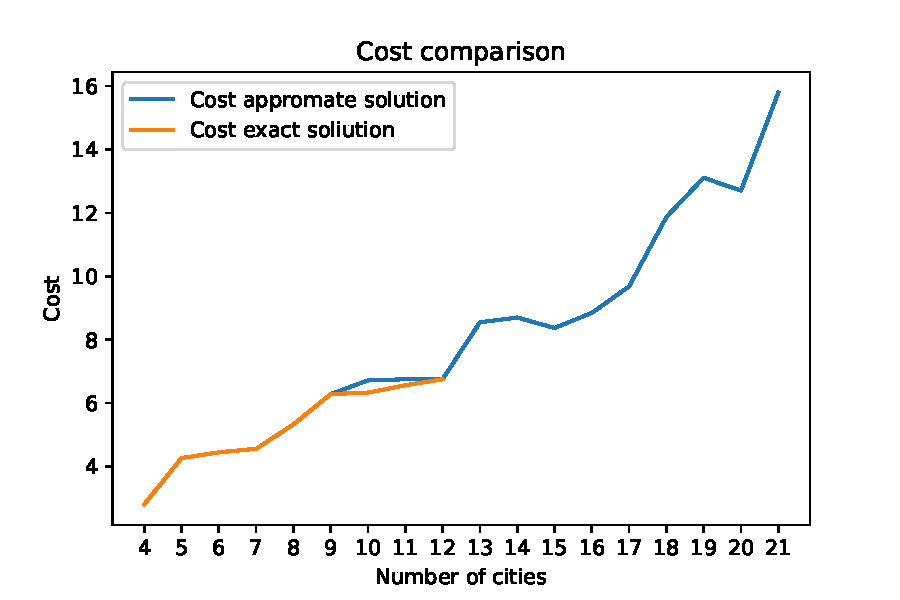
\includegraphics[width=0.60\textwidth]{../Cost_comparison.pdf} 
     }
     \hfill
     \subfloat{%
       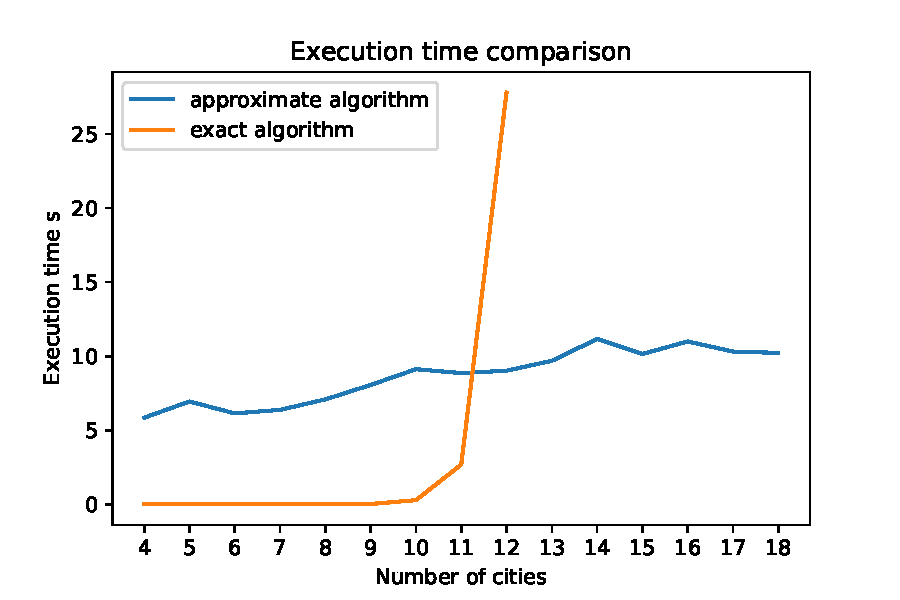
\includegraphics[width=0.60\textwidth]{../Time_comparison.pdf} 
     }
     
     \caption{Comparison between algorithms.}
    \end{adjustwidth}
   \end{figure}
 
\noindent As the plot above shows, simulated annealing is capable of finding optimal or slightly sub-optimal solutions. However, it is reasonable to expect that as the length of the cycles increases the optimal solutions of the simulated annealing move further away from the very best optimal solution. Since the algorithm is stochastic, can happen that longer cycles may have smaller cost than that of shorter cycles. For instance, the cost of the cycle with 13 cities is lower than the cost of the cycle with 12 cities.\\
In the following, it is plotted the shortest cycle computed by the simulated annealing when using all the possible cities. As mentioned before, the starting point is \textit{Varese}.
\begin{figure}[H]
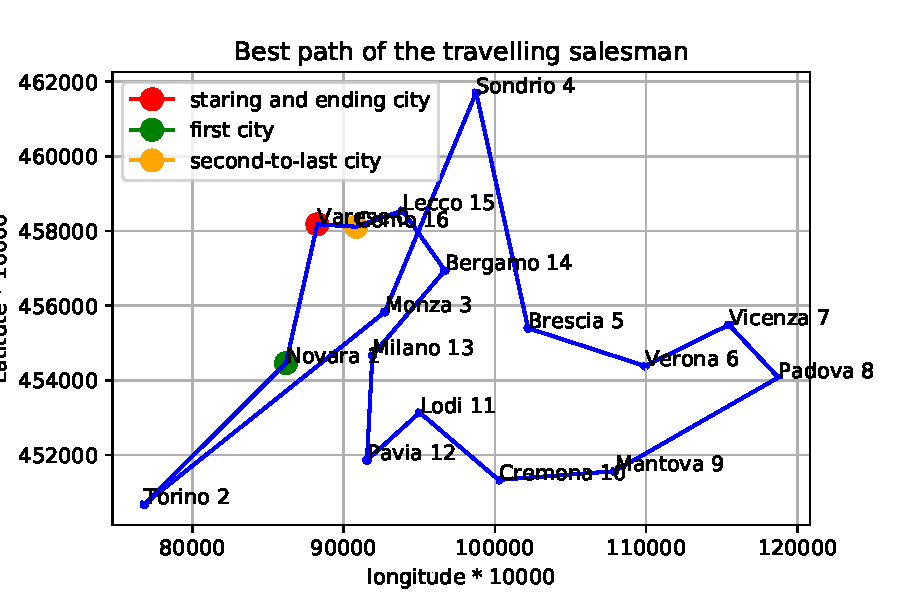
\includegraphics[scale=0.8]{../path.pdf} 
\centering
\caption{Optimal cycle starting from Varese}
\end{figure}

\section{Conclusion}
Overall, the simulated annealing and the genetic algorithm seem to have quite remarkable performance. The cost function is almost always increasing and as far as it is possible to compare the simulated annealing finds very optimal cycle while keeping the execution time very low. \\
As far as execution time is concerned, the length of the cycles seems to have a very limited influence on the execution time, indeed, it exhibits a very flat slope. \\
As for the optimal cycle computed, for all of the cities the euclidean distance provides a suitable approximation of the routes of the highways present in northern Italy. However, this notion of distance does not take into account the travel of the highways that can significantly change during the day and may not be correlated to significantly with the length of the highways. 

\newpage

\begin{thebibliography}{9}

\bibitem{metropolis}
Oliver Catoni
\textit{Simulated annealing algorithms and Markov chains with rare transitions}, Séminaire de probabilités (Strasbourg), tome 33 (1999), p. 69-119.

\bibitem{mctheory}
Marius Iosifescu
\textit{Finite markov process and their applications}, John Wiley \& Sons, 1980.

\bibitem{mcalgorithm}
M. Mitzenmacher, E. Upfal
\textit{ Probability and Computing}, Cambridge university Press, 2005.

\bibitem{gaBraun}
Heinrich Braun
\textit{On solving the travelling salesman problems by genetic algoritms}

\bibitem{gareview}
P. Larranaga, C.M.H. Kuijpers, R.H. Murga, I. Inza and S. Dizdarevic
\textit{Genetic Algorithms for the Travelling Salesman Problem: A Review of Representations and Operators}, Artificial Intelligence Review 13: 129–170, 1999.

\bibitem{annreview}
C. Peterson
\textit{Parallel Distributed Approaches to Combinatorial Optimization: Benchmark Studies on Traveling Salesman Problem}

\bibitem{test}
https://upload.wikimedia.org/wikipedia/commons/thumb/a/a0/P\_np\_np-complete\_np-hard.svg/2000px-P\_np\_np-complete\_np-hard.svg.png

\bibitem{autostrade}
http://www.autostrade.it/it/autostrade-per-genova?nomobile=true

 
\end{thebibliography}

\end{document}